\documentclass{article}
% Drop this file into the ICLR 2024 template folder (replace its main.tex) and
% compile on Overleaf or with pdflatex+bibtex. Requires the ICLR style files:
%   iclr2024_conference.sty, iclr2024_conference.bst, fancyhdr.sty, math_commands.tex
\usepackage{iclr2024_conference,times}
\input{math_commands.tex}

\usepackage{hyperref}
\usepackage{url}
\usepackage{graphicx}
\usepackage{booktabs}
\usepackage{amsmath}
\usepackage{xcolor}

\title{Condition, Don't Filter: \\ Quality-Conditioned Fine-Tuning of StyleGAN3 \\ for CelebV-HQ Face Generation}

\author{Heeyoon Lee \\
Ulsan National Institute of Science and Technology (UNIST) \\
\texttt{rlagkdus705@unist.ac.kr} \\ % replace with your own address if needed
}

\newcommand{\fix}{\marginpar{FIX}}
\newcommand{\new}{\marginpar{NEW}}

\iclrfinalcopy

\begin{document}
\maketitle

\begin{abstract}
We fine-tune an FFHQ-U pretrained \textbf{StyleGAN3-R} on frames from CelebV-HQ
and study how the \emph{quality} of training frames (brightness, sharpness)
should be handled. We compare three regimes that share an identical model,
optimizer, seed, and training length, differing only in how low-quality frames
are treated: (i) using the \textbf{full} set of frames, (ii) \textbf{filtering}
out dark/blurry frames, and (iii) keeping every frame but \textbf{conditioning}
the model on a brightness$\times$sharpness bucket label. Evaluated on the
challenge's four metrics (FID, IS, KID, TopP\&R) against the $32{,}550$-image
CelebV-HQ reference, filtering raises Inception Score but degrades all three
distribution-matching metrics, because the reference set is itself ``messy'' and
discarding modes pushes the generated distribution away from it. Conditioning,
in contrast, matches the full-data baseline on FID and TopP\&R while
\emph{improving} KID and IS, and additionally exposes a generation-time knob
(the bucket sampling proportions) that the baselines lack. All randomness is
seeded and the full pipeline is released for exact reproduction.
\end{abstract}

\section{Introduction}
The task is to generate $1{,}000$ face images that match the CelebV-HQ
distribution as measured by four metrics---Fr\'echet Inception Distance (FID;
\citealp{heusel2017fid}), Inception Score (IS; \citealp{salimans2016is}), Kernel
Inception Distance (KID; \citealp{binkowski2018kid}), and Topological Precision
and Recall (TopP\&R; \citealp{kim2023toppr})---averaged into a single rank. We
adopt the simplest competitive recipe: fine-tune an FFHQ-U pretrained
StyleGAN3-R generator \citep{karras2021alias} on CelebV-HQ frames
\citep{zhu2022celebvhq}, with no change to the architecture, loss, or training
algorithm.

Rather than chase architectural novelty, we focus on a single, practical
question that arises directly from the data: the extracted video frames vary
widely in \emph{quality}---many are dark or motion-blurred. A natural impulse is
to clean the training set by discarding such frames. We show this impulse is
counterproductive under the challenge's metrics, and that the same quality
information is better used as a \emph{conditioning signal} than as a filter.

Our contributions are: (1) a controlled three-way comparison (full / filtered /
conditional) in which only the data-handling strategy varies; (2) evidence that
filtering trades a single reference-free metric (IS) for losses on all three
distribution-matching metrics; (3) a quality-conditioned model that keeps the
full distribution while improving IS and KID over the plain baseline, with a
controllable generation-time proportion knob; and (4) a fully seeded, publicly
released pipeline built for exact reproduction.

\section{Method}
\subsection{Base model and fine-tuning}
All experiments fine-tune the public \texttt{stylegan3-r-ffhqu-256x256}
checkpoint at $256\times256$ using the official NVIDIA StyleGAN3 code with
adaptive discriminator augmentation (ADA; \citealp{karras2020ada}). We keep a
single fixed configuration across every run: \texttt{cfg=stylegan3-r},
generator channel base $32768$ / discriminator $16384$ (set via
\texttt{-{}-cbase=16384}; the configuration doubles the generator base
internally), $\gamma=2$, batch size $32$, one GPU, and random seed $0$. We train
each run for exactly $1{,}000$ kimg and select, \emph{per run}, the snapshot
with the lowest local \texttt{fid50k\_full}.

\subsection{Three data-handling regimes}
The three experiments are identical except for the training data:
\begin{itemize}
  \item \textbf{exp1 (full).} All $\sim\!35{,}610$ extracted frames, unconditional.
  \item \textbf{exp2 (filtered).} Frames below brightness/sharpness thresholds
        removed, leaving $12{,}403$ frames, unconditional. This operationalises
        the ``clean the data'' impulse.
  \item \textbf{exp3 (conditional).} The same full $\sim\!35{,}610$ frames as
        exp1, but each frame is labelled with a brightness$\times$sharpness
        bucket and the model is trained conditionally.
\end{itemize}
exp1 and exp3 use \emph{the same data}; exp3 only adds labels. exp2 is the
smaller filtered set. The contrast across the three isolates the effect of the
data-handling choice.

\subsection{Quality buckets and conditional generation}
\label{sec:cond}
We define quality along two axes computed identically for exp2 and exp3:
\textbf{brightness} (mean luma) and \textbf{sharpness} (variance of the
Laplacian, a standard blur measure). Splitting each axis at its median yields
four joint buckets:
$\{0\!:\text{dark+blurry},\,1\!:\text{dark+sharp},\,2\!:\text{bright+blurry},\,3\!:\text{bright+sharp}\}$.
On CelebV-HQ the two axes are strongly correlated: the realised bucket
proportions are $(0.366, 0.134, 0.134, 0.366)$---dark frames tend to be blurry
and bright frames tend to be sharp, with the off-diagonal buckets rare.

\paragraph{Conditional resume.}
The FFHQ-U checkpoint is unconditional, so a conditional model contains
label-embedding layers (the generator's first mapping layer and the
discriminator's label projection) with no counterpart in the checkpoint. We
therefore transfer every shape-matching tensor---i.e.\ essentially the entire
synthesis network and all learned image-quality knowledge---and randomly
initialise only the label-specific layers, which the model then learns during
fine-tuning. This is the only modification to the upstream code and is a no-op
for the unconditional runs.

\paragraph{Proportional sampling.}
At generation time, a conditional model requires a label per image. We draw the
per-image bucket from a fixed-seed sampler according to a proportion vector
$\mathbf{p}$. Setting $\mathbf{p}$ to the training proportions matches the
reference distribution; biasing it toward the sharp buckets trades diversity for
Inception Score. This proportion vector is a controllable knob that the
unconditional baselines do not have.

\section{Experimental Setup}
\paragraph{Data.}
Frames are extracted from CelebV-HQ videos to $256\times256$ crops. A pilot
diagnosis of the extracted frames found a large fraction to be dark or blurry,
which motivates the quality study. The filtered set (exp2) retains $12{,}403$ of
$35{,}610$ frames.

\paragraph{Metrics.}
We report the four challenge metrics computed against the full $32{,}550$-image
CelebV-HQ reference from $1{,}000$ generated images. Lower is better for FID and
KID; higher is better for IS and TopP\&R. We additionally track
\texttt{fid50k\_full} ($50{,}000$ samples) \emph{locally} during training for
snapshot selection only; note that the local and leaderboard FID are not
directly comparable, largely because FID is biased upward at the small
($1{,}000$) sample size used for scoring.

\paragraph{Reproducibility.}
Training uses seed $0$; generation uses the fixed seed range $0$--$999$; for the
conditional model the per-image bucket assignment uses a fixed label seed. The
exact environment is pinned (notably \texttt{face-alignment==1.3.5},
\texttt{ninja}, and the CUDA-matched PyTorch~1.12.1 build), and the full
pipeline---preprocessing, training scripts, the conditional-resume patch,
inference, and submission packaging---is released publicly
(Section~\ref{sec:repro}).

\section{Results}
\subsection{Main comparison}
Table~\ref{tab:main} reports the four leaderboard metrics. The three runs share
model, seed, and training length ($1{,}000$ kimg), and each uses its
lowest-local-FID snapshot (exp1: $960$; exp2: $760$; exp3: $1000$ kimg).

\begin{table}[h]
\centering
\caption{Leaderboard metrics ($1{,}000$ generated images vs.\ the
$32{,}550$-image CelebV-HQ reference). Best per column in \textbf{bold}.
Arrows indicate the favourable direction.}
\label{tab:main}
\begin{tabular}{lcccc}
\toprule
Experiment & FID $\downarrow$ & IS $\uparrow$ & KID $\downarrow$ & TopP\&R $\uparrow$ \\
\midrule
exp1 -- full (unconditional)        & \textbf{37.06} & 3.81 & 0.0089 & \textbf{0.8989} \\
exp2 -- filtered (unconditional)    & 42.99 & \textbf{4.49} & 0.0134 & 0.7718 \\
exp3 -- conditional (full + labels) & 37.27 & 3.90 & \textbf{0.0082} & 0.8887 \\
\bottomrule
\end{tabular}
\end{table}

\subsection{Snapshot selection}
Locally, the best \texttt{fid50k\_full} values are $7.64$ (exp1, $960$ kimg),
$10.73$ (exp2, $760$ kimg), and $7.88$ (exp3, $1000$ kimg). The full-data and
conditional runs reach a comparable local optimum, while the filtered run
plateaus markedly higher---an early signal of the effect confirmed on the
leaderboard. The local FID ordering (exp1 $<$ exp3 $<$ exp2) matches the
leaderboard FID ordering, supporting our snapshot choices.

\subsection{Qualitative comparison}
Figure~\ref{fig:grid} shows $16$ samples from each model at the same seeds. The
full and conditional models produce comparably clean, varied faces; the filtered
model's samples are individually sharp (consistent with its higher IS) but show
visibly reduced variation.

\begin{figure}[h]
\centering
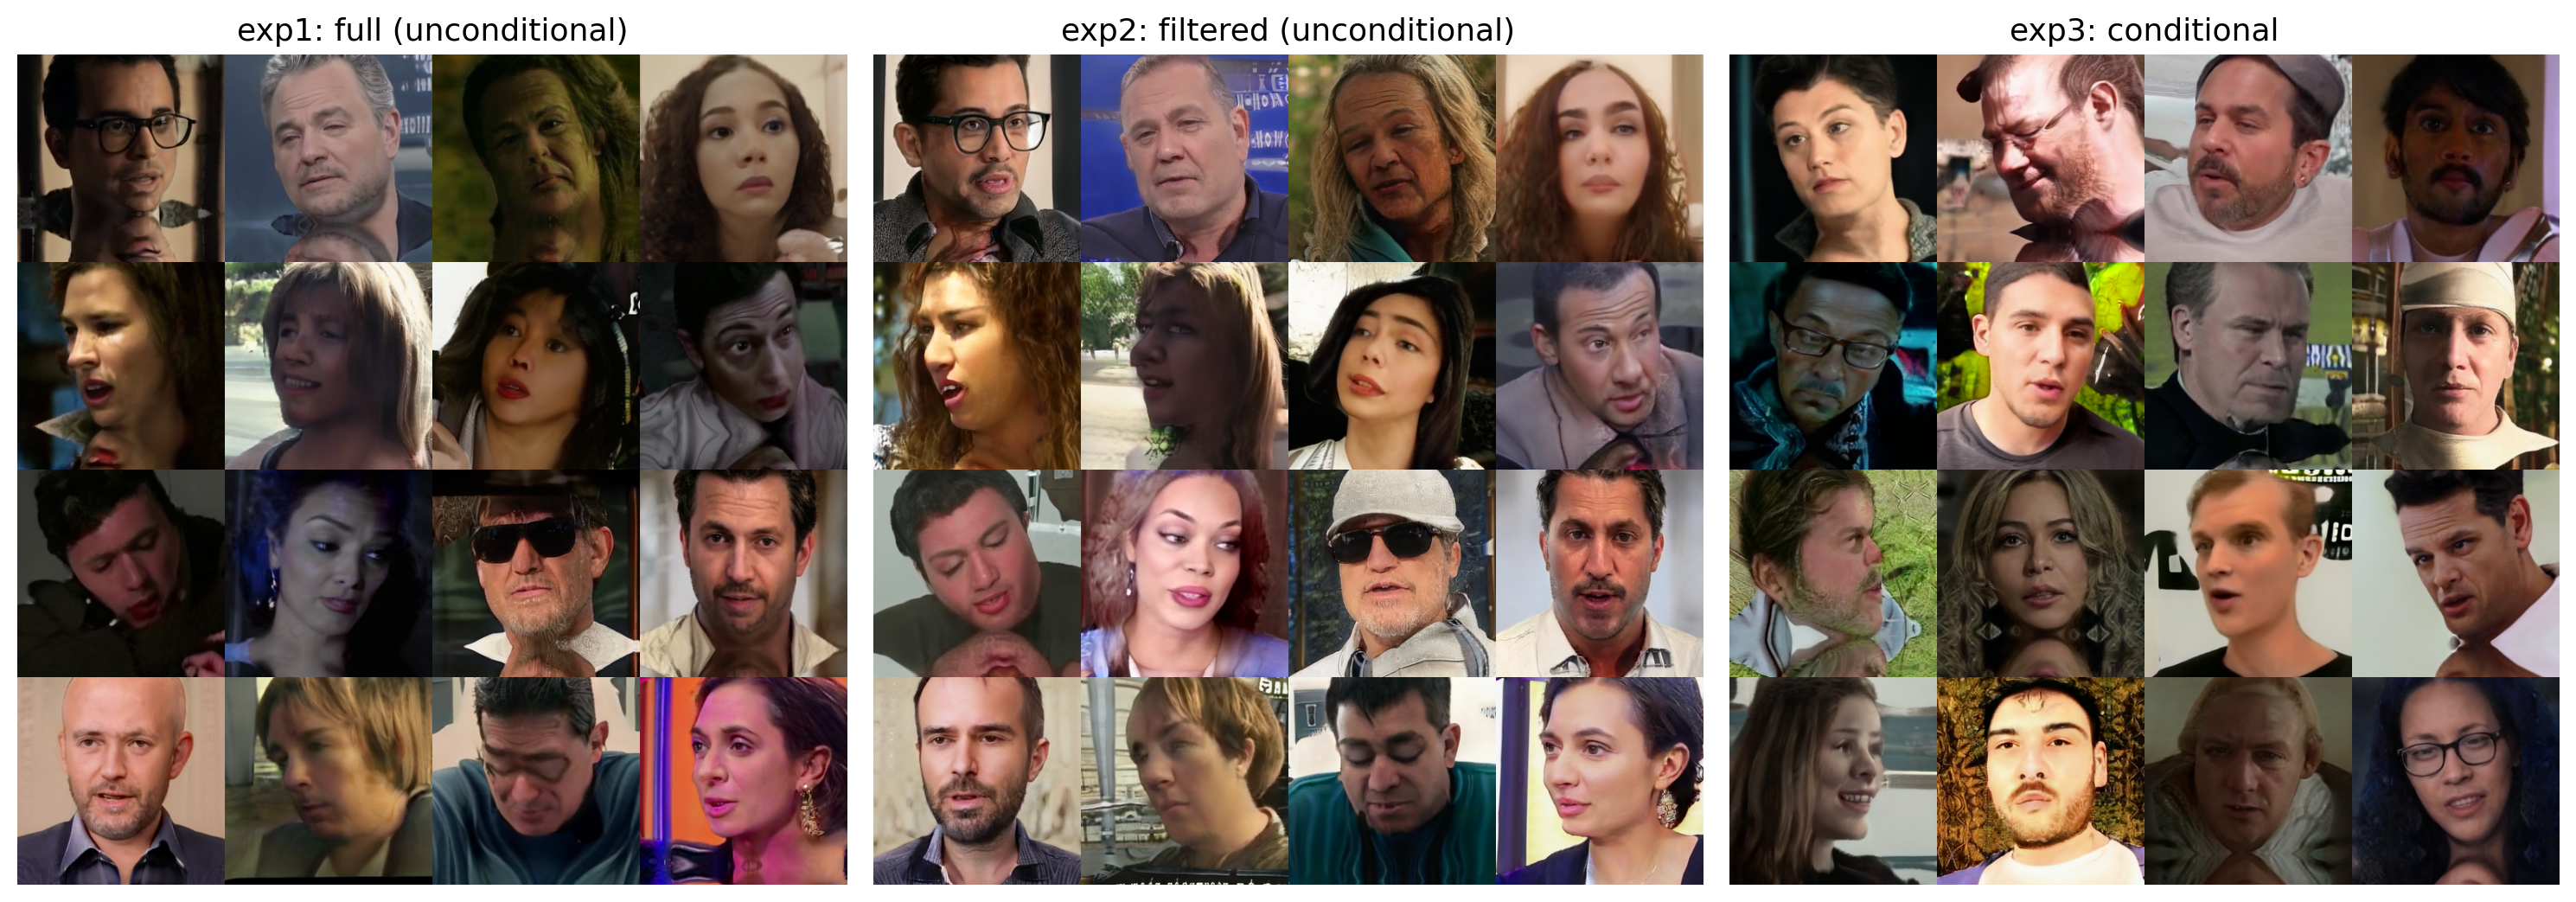
\includegraphics[width=\linewidth]{figures/comparison_grid.png}
\caption{Uncurated samples (16 per model, identical seeds). Left: exp1 (full).
Middle: exp2 (filtered). Right: exp3 (conditional).}
\label{fig:grid}
\end{figure}

\subsection{Analysis}
\paragraph{Filtering trades distribution match for sharpness.}
exp2 attains the best IS ($4.49$) but the worst FID, KID, and TopP\&R. The
mechanism is that the evaluation compares against the \emph{full, messy}
CelebV-HQ distribution. Three of the four metrics reward matching that
distribution, including its dark and blurry modes; only IS is reference-free and
rewards per-image confidence/diversity regardless of the target. Removing
low-quality frames makes the generator unable to reproduce those modes, so the
generated distribution drifts away from the reference (higher FID/KID) and loses
coverage (TopP\&R drops from $0.90$ to $0.77$). The IS gain is real but is the
only metric that benefits, and it is outweighed three-to-one.

\paragraph{Conditioning uses the quality signal without discarding modes.}
exp3 keeps every frame and instead conditions on quality. It matches the
full-data baseline on the distribution-matching metrics (FID $37.27$ vs.\
$37.06$; TopP\&R $0.8887$ vs.\ $0.8989$---both far above the filtered run) while
\emph{improving} KID ($0.0082$, best overall) and IS ($3.90$ vs.\ $3.81$) over
exp1. In other words, conditioning recovers part of the per-image quality that
filtering chased, but without the catastrophic distribution and coverage losses,
because the full set of modes is retained and merely organised by label. This
supports the central claim: the quality of frames is information to
\emph{condition on}, not to \emph{filter by}.

\section{Discussion}
\paragraph{The proportion knob.}
Because exp3 is conditional, the generation proportions $\mathbf{p}$ are a free,
post-hoc control. We report $\mathbf{p}$ set to the training proportions, which
matches the reference. Biasing $\mathbf{p}$ toward the sharp buckets is expected
to raise IS at some cost to coverage; given the comfortable TopP\&R margin, this
is a promising direction for squeezing additional rank without retraining. The
unconditional baselines offer no comparable control beyond truncation.

\paragraph{Local vs.\ leaderboard FID.}
Our local \texttt{fid50k\_full} ($\approx 7.6$ at best) is far below the
leaderboard FID ($\approx 37$). This gap is expected and largely structural: the
leaderboard scores only $1{,}000$ images, and FID is biased upward at small
sample sizes, whereas the local metric uses $50{,}000$. The two should therefore
be used for relative, not absolute, comparison; we rely on local FID only for
within-run snapshot selection, where the bias is shared.

\paragraph{Limitations.}
Local FID need not perfectly predict leaderboard rank, so the selected snapshots
may be slightly suboptimal on the $1{,}000$-image metric. We use a coarse
$2\times2$ quality bucketing; a finer grid or continuous conditioning could
sharpen the effect but risks under-populating rare buckets. Bit-exact
reproduction is not guaranteed across hardware due to floating-point
non-determinism; we mitigate this by releasing the exact weights
(Section~\ref{sec:repro}).

\section{Conclusion}
Across a controlled comparison that varies only the handling of frame quality,
filtering low-quality frames improves a single reference-free metric while
harming every distribution-matching metric, whereas conditioning on quality
preserves the full distribution and improves KID and IS over the plain baseline,
with a controllable generation-time knob. For matching a messy target
distribution, the right move is to condition on quality rather than filter by it.

\section*{Reproducibility Statement}
\label{sec:repro}
The complete pipeline is released at a public repository and is built for exact
reproduction. Training uses random seed $0$; image generation uses the fixed
seed range $0$--$999$ at truncation $\psi=1.0$; the conditional model additionally
fixes the per-image bucket-sampling seed and uses proportions
$(0.366, 0.134, 0.134, 0.366)$. The conda environment is pinned in
\texttt{environment.yml}, the upstream StyleGAN3 code is used with a single
documented patch (conditional resume), and the trained snapshot weights used for
each leaderboard submission are released so that the exact $1{,}000$ images can
be regenerated from the submitted code and weights. The exact per-experiment
generation commands are documented in the repository \texttt{README}.

\bibliographystyle{iclr2024_conference}
\begin{thebibliography}{}

\bibitem[Bi\'nkowski et al.(2018)]{binkowski2018kid}
Miko\l{}aj Bi\'nkowski, Dougal J. Sutherland, Michael Arbel, and Arthur Gretton.
\newblock Demystifying MMD GANs.
\newblock In \emph{International Conference on Learning Representations (ICLR)}, 2018.

\bibitem[Heusel et al.(2017)]{heusel2017fid}
Martin Heusel, Hubert Ramsauer, Thomas Unterthiner, Bernhard Nessler, and Sepp Hochreiter.
\newblock GANs trained by a two time-scale update rule converge to a local Nash equilibrium.
\newblock In \emph{Advances in Neural Information Processing Systems (NeurIPS)}, 2017.

\bibitem[Karras et al.(2020)]{karras2020ada}
Tero Karras, Miika Aittala, Janne Hellsten, Samuli Laine, Jaakko Lehtinen, and Timo Aila.
\newblock Training generative adversarial networks with limited data.
\newblock In \emph{Advances in Neural Information Processing Systems (NeurIPS)}, 2020.

\bibitem[Karras et al.(2021)]{karras2021alias}
Tero Karras, Miika Aittala, Samuli Laine, Erik H\"ark\"onen, Janne Hellsten, Jaakko Lehtinen, and Timo Aila.
\newblock Alias-free generative adversarial networks (StyleGAN3).
\newblock In \emph{Advances in Neural Information Processing Systems (NeurIPS)}, 2021.

\bibitem[Kim et al.(2023)]{kim2023toppr}
Pum Jun Kim, Yoojin Jang, Jisu Kim, and Jaejun Yoo.
\newblock {TopP\&R}: Robust support estimation approach for evaluating fidelity and diversity in generative models.
\newblock In \emph{Advances in Neural Information Processing Systems (NeurIPS)}, 2023.

\bibitem[Salimans et al.(2016)]{salimans2016is}
Tim Salimans, Ian Goodfellow, Wojciech Zaremba, Vicki Cheung, Alec Radford, and Xi Chen.
\newblock Improved techniques for training GANs.
\newblock In \emph{Advances in Neural Information Processing Systems (NeurIPS)}, 2016.

\bibitem[Zhu et al.(2022)]{zhu2022celebvhq}
Hao Zhu, Wayne Wu, Wentao Zhu, Liming Jiang, Siwei Tang, Li Zhang, Ziwei Liu, and Chen Change Loy.
\newblock {CelebV-HQ}: A large-scale video facial attributes dataset.
\newblock In \emph{European Conference on Computer Vision (ECCV)}, 2022.

\end{thebibliography}

\end{document}
